\documentclass[12pt, letterpaper]{article}

\usepackage{graphicx}

\title{How2HotShot: A Guide to Operating the Hot Shot Electric Boiler for Teaching Assistants}
\author{Joshua Holbrook}

\begin{document}

\maketitle

\begin{figure}
\label{fig:boiler}
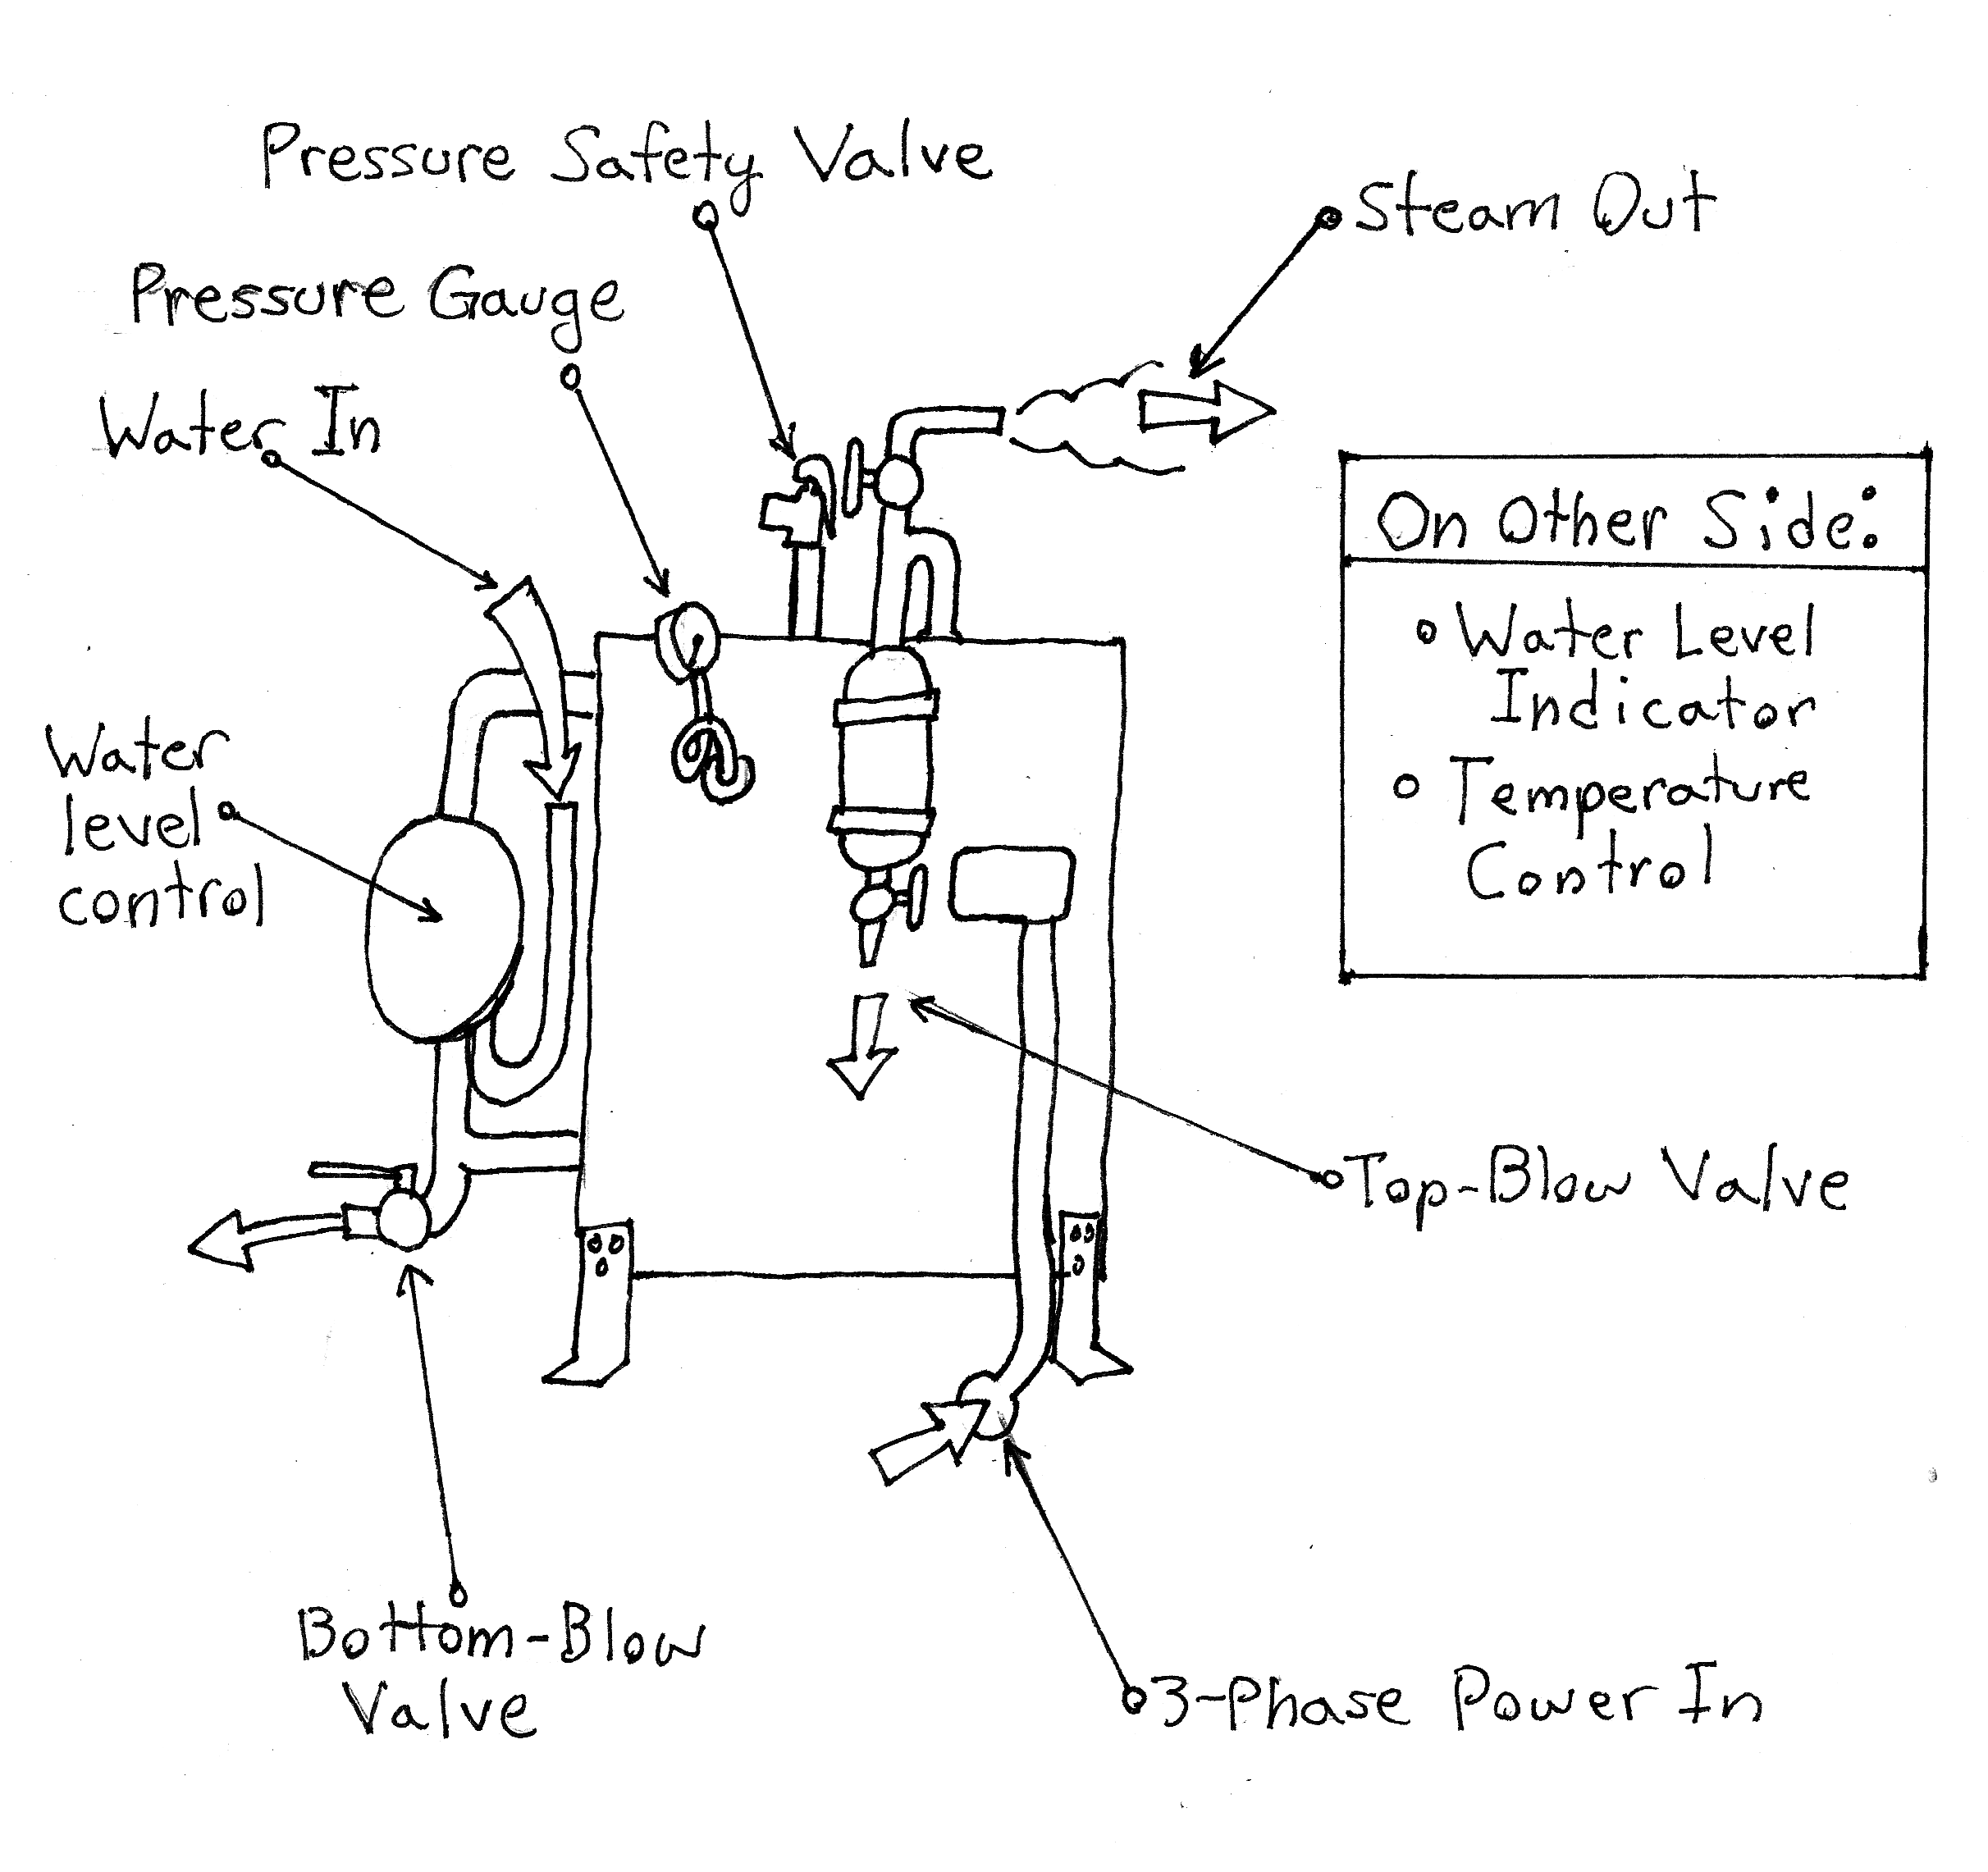
\includegraphics[width=0.9\textwidth]{boiler}
\caption{A sketch of the Hot Shot boiler, with important parts labelled.}
\end{figure}

The boiler, conceptually, is actually quite simple. It uses electric heating elements to boil water. Water is supplied with a hose, and hot steam comes out.

The water level is controlled by what is labelled as the ``water level control'' in Figure \ref{fig:boiler}. Think of it kinda like a toilet float.


\end{document}
